% Mihir Savadi | 27-Apr-2022 

% TODO: add github links as footnotes to all relevant places especially in section 4 and 5.

% TODO: CTRL-F all TODOs in document and complete

\documentclass[10pt,twocolumn,letterpaper]{article}

\usepackage{cvpr}
\usepackage{times}
\usepackage{epsfig}
\usepackage{graphicx}
\usepackage{amsmath}
\usepackage{amssymb}
% Include other packages here, before hyperref.
\usepackage[ type={CC}, modifier={by-nc-sa}, version={4.0}, ]{doclicense} % for licensing

\newcommand*\diff{\mathop{}\!\mathrm{d}} % helps makes typesetting calculus notation easier
\newcommand*\Diff[1]{\mathop{}\!\mathrm{d^#1}} % same as above but anything right after is a superscript

% If you comment hyperref and then uncomment it, you should delete egpaper.aux before re-running latex.  (Or just hit
% 'q' on the first latex run, let it finish, and you should be clear).
\usepackage[breaklinks=true,bookmarks=false]{hyperref}

\cvprfinalcopy % *** Uncomment this line for the final submission

\def\cvprPaperID{****} % *** Enter the CVPR Paper ID here
\def\httilde{\mbox{\tt\raisebox{-.5ex}{\symbol{126}}}}

% Pages are numbered in submission mode, and unnumbered in camera-ready \ifcvprfinal\pagestyle{empty}\fi
\setcounter{page}{1}
\begin{document}

    \title{A Neural-Network Based Real-Time SISO Controller:\\Real-Time Convergent Feedback Loop (RTCFL)}

    \author{Mihir Savadi\\
    Bradley Department of Electrical and Computer Engineering\\
    Virginia Tech\\ \today\\
    {\tt\small mihirsavadi1@vt.edu} }

    \maketitle
    \thispagestyle{empty}

    \begin{abstract} 
        PID control feedback loops are truly ubiquitous amongst a wide variety of controls and automation processes in
        the modern world. However, before being released, in order to achieve adequate performance, they require manual
        tuning by a human with domain specific knowledge. This paper proposes the Real-Time Convergent Feedback Loop
        (RTCFL) -- a generally applicable approach that converges upon good control performance of any system over time
        without human input, whilst being risk-averse enough to be trained online and in real-time. In addition, the
        `Control-Feedback Testbench' (CFT) -- a software environment for simulation of control-feedback loops -- is
        showcased.
        % TODO include CODEBASE github link - reference to github
    \end{abstract}
    \tableofcontents

    \section{Introduction} \label{intro}

        PID (potential, integral, derivative) control loops are ubiquitous in our world today -- it is the de-facto
        control mechanism behind ovens, toasters, home or auto HVACs, cruise controls, auto pilots, attitude control in
        drones, and various industrial processes. Its popularity is due to its simplicity, reliability, and
        interpretability -- it has been commonplace in industry for several decades. One drawback of the PID control
        mechanism is that the parameters that govern them require manual human tuning via trial and error. In many
        applications this may be inconvenient or costly. This paper proposes an approach that, for any system (or plant)
        thrown under its purview, can automatically converge upon equivalent behavior of an ideally tuned PID control
        loop (i.e. achieve perfect damping\footnote{\url{https://en.wikipedia.org/wiki/Damping} \label{wikidamp}}),
        given real-time data fed to it from the system/plant it is controlling, and no human input. The architecture of
        this approach will be referred to as the Real-Time Convergent Feedback Loop (RTCFL).

        For those unfamiliar, the basics of PID controller's will be outlined -- they are remarkably simple. Motivations
        for this project will then be explained, before covering the architecture of the software testbench that was
        built in order to efficiently and scalably facilitate the simulation and testing of any arbitrary
        controller-plant circuit. Finally, the architecture of the RTCFL will be discussed and its performance
        evaluated.
        % TODO include CODEBASE github link

    \section{PID Controllers Explained} \label{pidexplained}

        Say we had an oven that we wanted to control the temperature of. The intended temperature can be set to any
        value in a given range by a cook, and the actual temperature of the oven would then be influenced by a heating
        coil within it. This heating coil would be controlled by some electrical circuitry (often times
        mechanical!\footnote{Bimetallic strips are commonly found controlling car blinkers -- making sure their
        switching frequency is constant; or the temperature control in mini-fridges.}) that would carefully alter the
        power of the heating coil such that a steady temperature is maintained. If the oven is already at a steady
        temperature, and the cook increases the intended temperature, the controller would then be responsible for
        ramping up power of the coil so that the oven is able to settle at the new temperature quickly, but not
        overshoot or oscillate around it (i.e. it must ensure a \textit{perfectly damped}\footnotemark[1] response). The
        inverse of the same logic applies if the cook decreased the temperature instead.

        In this example, our oven is our system that we are concerned about, which we will refer to as the
        \textbf{plant}. The output characteristic of our plant that we wish to control is the temperature, which varies
        with time -- we will refer to it as $y(t)$. The input to our plant that our controller control's in order to
        influence $y(t)$ is the power of the heating coil, which also varies with time -- we will refer to it as $u(t)$.
        The intended value of $y(t)$ -- as decided by any agent, in our example the cook sets an intended temperature --
        can also vary with time and will be referred to as $r(t)$. The error between the intended and the actual plant
        output will be referred to as $e(t)$. Eq~\ref{pideq} defines a PID controller.
        
        \begin{equation} \label{pideq}
            \begin{gathered}
                u(t) = K_P e(t) + K_I \int_0^t e(\tau) \diff\tau + K_D \frac{\diff e(t)}{\diff t} \\
                \text{where } e(t) = r(t) - y(t)
            \end{gathered}
        \end{equation}
        
        In Section~\ref{intro} we mentioned how PID controllers have parameters that require manual tuning -- these are
        $K_P$ (called the potential), $K_I$ (called the integral), and $K_D$ (called the derivative), which can be seen
        in Eq~\ref{pideq}. Figure~\ref{pidblock} is a block diagram representation of Eq~\ref{pideq}, which should help
        illustrate the real-time nature of this type of system. It can be observed that PID controllers are Single-Input
        Single-Output systems (SISO).
        
        \begin{figure}[h]
            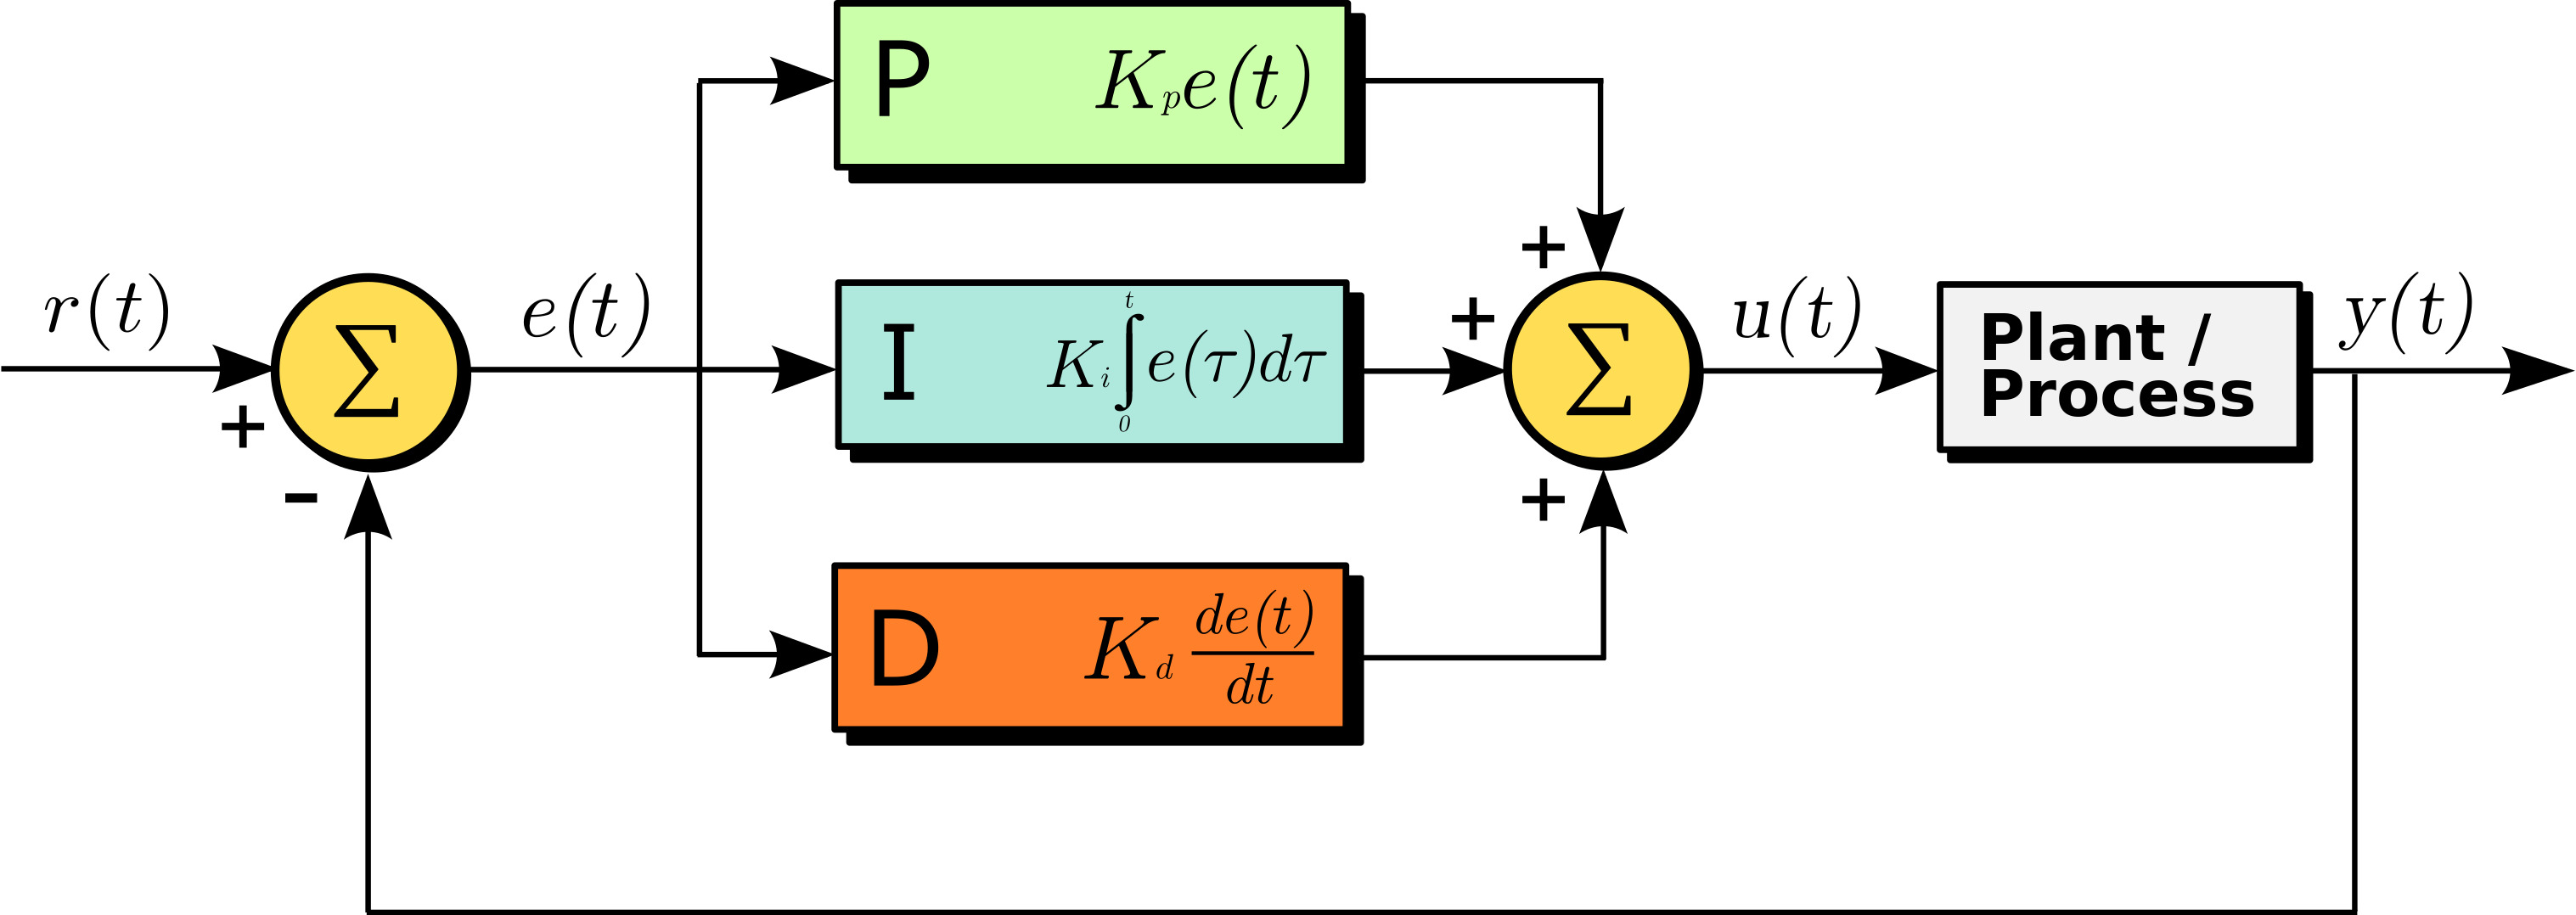
\includegraphics[width=\linewidth]{./figures/pidBlock.jpg}
            \centering
            \caption{Block diagram of a PID controller.\cite{wikipediaPIDdiagram}}
            \label{pidblock}
        \end{figure}

        Considering that we will be operating in discrete time due to the digital nature of our computational platforms,
        Eq~\ref{pideq_discrete} below is the `digital' version of Eq~\ref{pideq}.
        
        \begin{equation} \label{pideq_discrete}
            \begin{gathered}
                u[t] = K_P e[t] + K_I \sum_{i=0}^n e[t-i] + K_D \left(e[t]-e[t-1]\right) \\
                \text{where } e[t] = r[t] - y[t], \text{and $n \geq 0$}
            \end{gathered}
        \end{equation}

    \section{Motivation} \label{motivation}
        
        In certain situations, relying on PID control systems to achieve control stability is impractical. A common
        example would be when one-off systems, that aren't massed produced and don't have R\&D time before mass
        production, need to be tuned. For example, whenever an amateur racing drone pilot builds a new custom drone with
        an off-the-shelf flight controller, they then assume the burden of tuning the PID parameters that govern their
        drone's flight characteristics. This involves flying around, observing flight behavior, and tuning iteratively
        via trial-and-error -- this is clearly cumbersome and can even lead to situations that may damage this one-off
        drone. Modern flight control software comes with auto-tuning features, but these are mostly deterministic and
        perform poorly.

        Another example would be DIY reflow ovens. When hobbyists or independent printed circuit board designers want to
        build large complex boards or boards with several hard-to-hand-solder surface mount devices, they often seek the
        refuge of `reflow-ovens'. The reflow oven process involves a PCB with components placed onto their footprints
        with unsoldered `solder paste' in between. This PCB is then placed into a reflow oven, which controls the
        temperature in its chamber to follow a very specific temperature-time curve in order for the solder paste to
        melt and create sound solder joints as per the manufacturers specifications. Often times hobbyists modify
        toaster ovens into reflow ovens (which are very popular and work remarkably well) by swapping out existing cheap
        mechanical controls with their own programmed PID controllers, which they then have to tune. If instead they
        could use an auto-tuning `adaptive' controller, it would make the conversion process of any randomly chosen
        toaster oven a lot easier.

        Similar arguments from the examples above can be used to justify the benefits of such an `adaptive' controller
        in various industrial applications. As such, many efforts have already been made and are currently even being
        used in deep industry (see references), however many remain seemingly proprietary. The RTCFL approach (detailed
        in Section~\ref{RTCFLexpained}) is not one that has been explicitly observed yet in existing literature.
        
    \section{Control-Feedback Testbench Architecture} \label{tbarch}

        In order to efficiently build, analyze, and maintain a variety of control-feedback circuit designs without
        compromising design flexibility and granularity, the use of a modular `testbench' environment/platform was
        imperative. Such a testbench, simply referred to as the `Control-Feedback Testbench' (or CFT), was built as such
        to facilitate the exploration of the RTCFL proposed in this paper. Hopefully, by the end of this section the
        reader will recognize it's utility beyond just the scope of this paper.

        The testbench implemented is fundamentally modular, employing object orientated design with heavy use of both
        inheritance (to enforce inter-class communication consistency without compromising modularity) and composition.
        At its core, the testbench is based on the `actor' paradigm, whereby each element in any given circuit (e.g. in
        Figure~\ref{pidblock} or \ref{rtcflcircuit} for example) is treated as a black box, or an actor, whose basic
        inputs and outputs are standardized by an abstract actor base class, and whose internal calculations are
        abstracted away. Actors can be controllers, plants, or any other influencing element of a circuit. 
        
        Actor objects are then instantiated inside a circuit class, which contain standardized inputs and outputs
        themselves, and abstract away the interconnections (whether chronological or parallel) between whatever actors
        may be present in said particular circuit. These standardizations are again enforced by an abstract circuit base
        class. Circuit classes contain a single function to update actor outputs according to its defined
        interconnections for each time-step, as well as store historical data for each `wire' in the circuit.
        
        Finally, a scheduler class is what the user interacts with in order to utilize the testbench -- it contains an
        instance of a particular circuit class, whose parameters are determined on initialization of a scheduler object;
        it provides a function to get inputs into the circuit, either by time-step by time-step polling or by parsing an
        external text file; it provides a function to probe the circuit to get information on its stored current and
        historical data; and it provides a function to generate a convenient plot to quickly visualize circuit behavior,
        e.g. Figure~\ref{controllertboutputplot}, ??, ??, ??.
        
        \begin{figure}[h]
            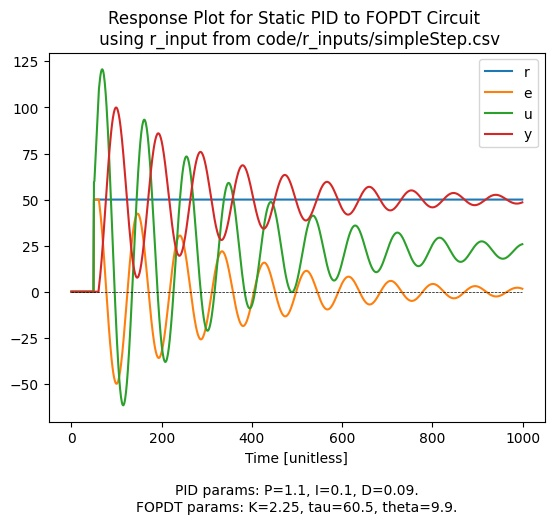
\includegraphics[width=\linewidth]{./figures/output_plot_2022Apr25221020.jpg}
            \centering
            \caption{Example output plot generated by the CFT for a simple PID controller + FOPDT plant, where the PID
                controller is not well tuned -- the control-feedback loop is under damped. Refer to fig~\ref{pidblock}
                for plot label references.}
            \label{controllertboutputplot}
        \end{figure}

        The user can create arbitrary actor classes (controllers, plants, etc.) and circuit classes, which will function
        predictably with the aforementioned scheduler class, as long as the respective abstract base classes are adhered
        to. Thus, a user can use the scheduler class of this testbench to automate testing and analysis of a variety of
        controllers, plants, and circuits, in an arbitrarily simulated real-time environment.

        % TODO talk about where codebase can be found -- github link, and the RTCFL actors use pytorch.

    \section{The RTCFL Approach} \label{RTCFLexpained}

        In order to understand the RTCFL approach, the interconnects between each actor in the circuit shown in
        Figure~\ref{rtcflcircuit} must first be studied. As is almost immediately obvious, the RTCFL is model-based.
        Section~\ref{RTCFLarch} walks through the RTCFL approach step-by-step, and Section~\ref{RTCFLtesting} evaluates
        its performance.

        \begin{figure}[h]
            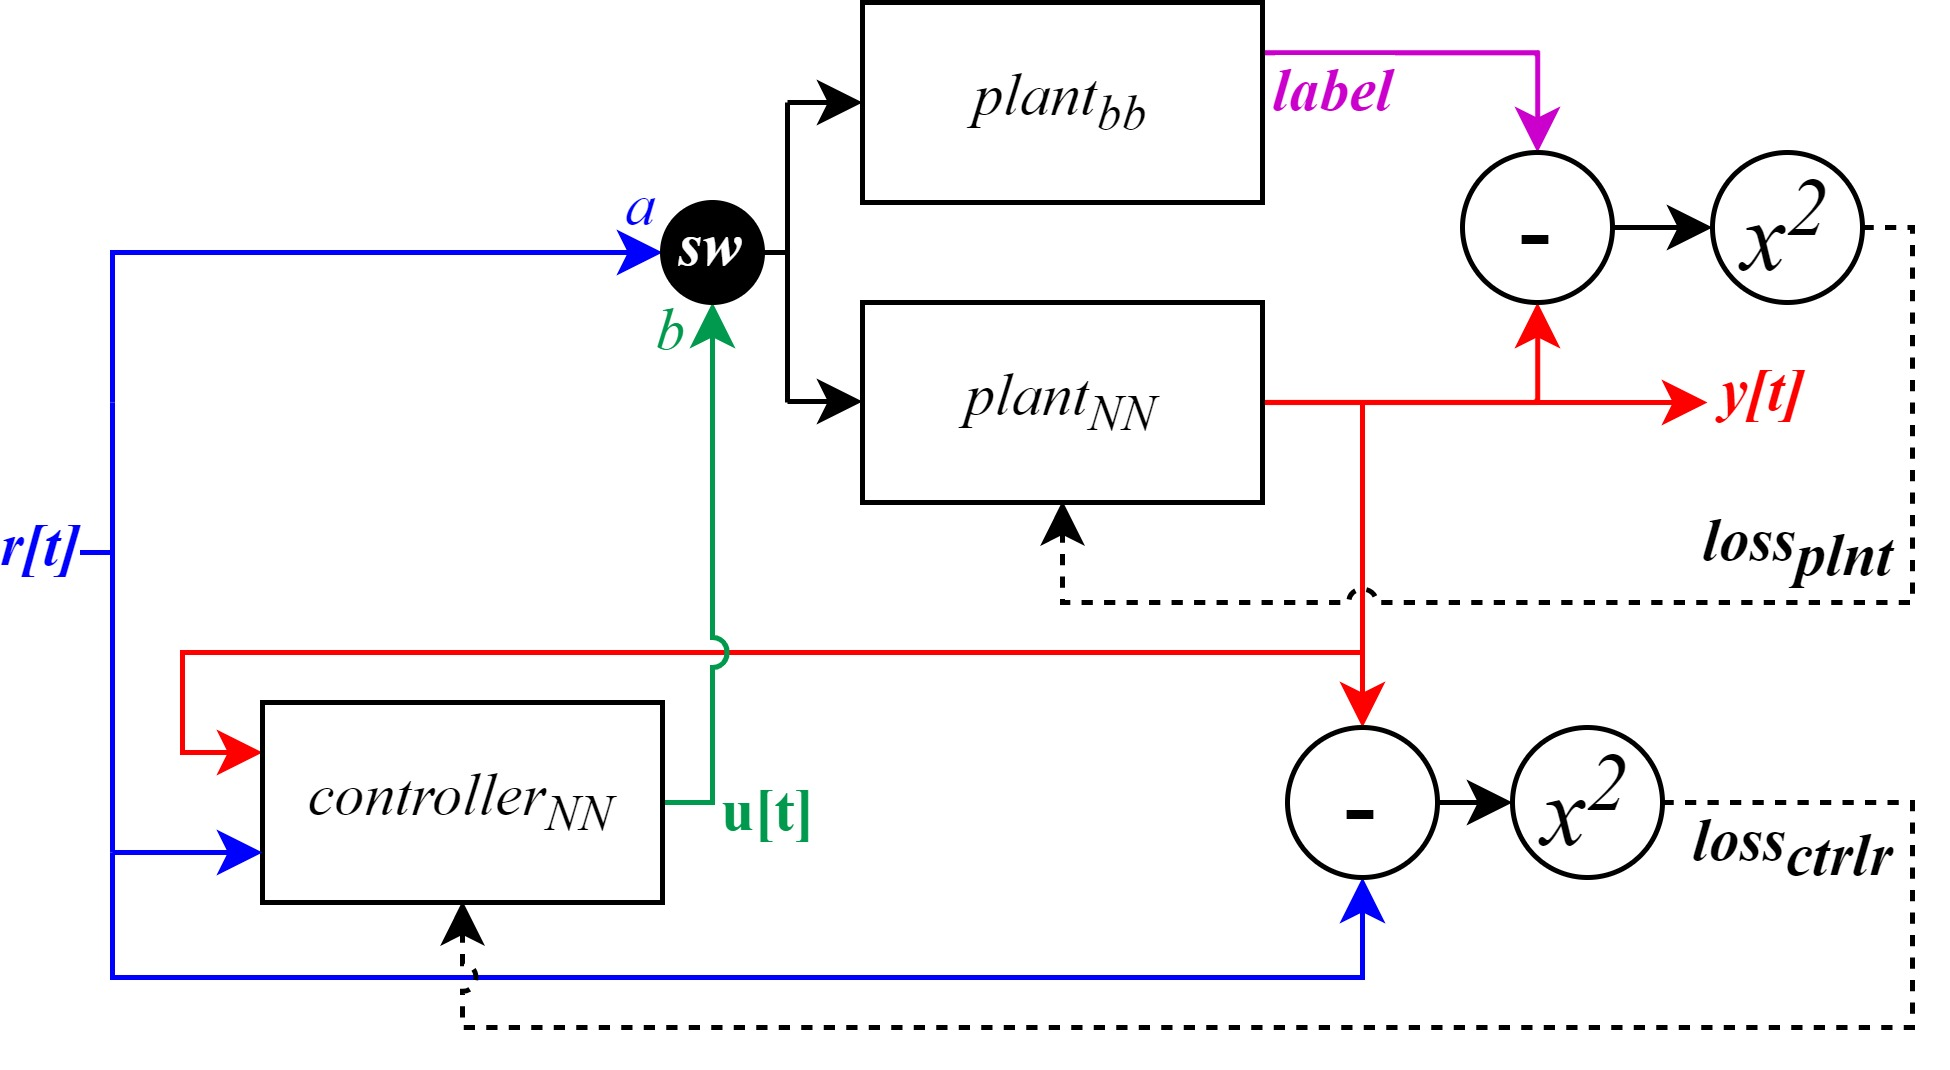
\includegraphics[width=\linewidth]{./Figures/rtcfl-circuit.jpg}
            \centering
            \caption{RTCFL circuit diagram. Each square box represents an actor: plant\textsubscript{bb} is the original
                black-box plant that plant\textsubscript{NN} seeks to emulate; controller\textsubscript{NN} is the NN
                that ultimately needs to be trained to achieve optimal plant control. Each actor can either be `dormant'
                or `active' from the point of view of the circuit. The NN based actors handle and switch between
                `learning' and `inference' modes within themselves. The black circle labelled `SW' acts as a switch
                redirecting either the \textcolor{blue}{$r[t]$ vector on its $a$ channel} or the \textcolor{teal}{$u[t]$
                vector on its $b$ channel} into both the plants. The \textcolor{blue}{$r[t]$}, \textcolor{teal}{$u[t]$},
                \textcolor{red}{$y[t]$} vectors follow the convention shown in Fig~\ref{pidblock}. The black dotted
                vectors indicate objective function output values used to train their respective NN's via gradient
                descent.}
            \label{rtcflcircuit}
        \end{figure}

        \subsection{High Level Architecture} \label{RTCFLarch}

            Refer to the description of Figure~\ref{rtcflcircuit} for a basic explanation of the function of each
            element in the circuit shown. The steps below will outline the series of operations within the circuit that
            defines the RTCFL approach. Note that $plant_{NN}$ exists to enable training of $controller_{NN}$ in later
            steps of the RTCFL approach via backpropagation, by providing a known function through which the derivative
            of the loss function with respect to the parameters of $controller_{NN}$ can be calculated -- this would not
            be possible with the `black box' that is $plant_{bb}$, where it's inner function is unknown. 
            
            Just for the sake of simulation testing $plant_{bb}$ is initialized as an arbitrary FOPDT (first order plus
            dead time) model. The RTCFL circuit was tested with $plant_{NN}$ and $controller_{NN}$ being implemented as
            DNN's in one instance (with inputs being a fixed vector of up to [t-n] time series data), and RNN's in
            another. Their architectures can as such be experimented with without altering overall RTCFL approach -- the
            CFT enables this flexibility.

            \textbf{Step 1}\\
            $SW$ is set to pass its $a$ signal and block its $b$ signal. $controller_{NN}$ is disabled, $plant_{bb}$ and
            $plant_{NN}$ (initialized with random weights) are enabled.

            $r[t]$ signals are chosen with enough temporal variation to encapsulate what is typical of whatever the
            chosen application space is. These are then passed concurrently into both plants, whereby $plant_{bb}$'s
            output is treated as a label, against which $plant_{NN}$'s output is used to calculate a loss value --
            $loss_{plnt}$.

            As time goes on, an internal data base is appended to with $r[t]$ time series data (with a variable `n'
            number of time-steps into the past), along with associated $y[t]$ and $label$ (that is $plant_{bb}$'s
            output) data. The interval with which this happens is flexible. Then, at another variable-number of time
            steps, this data base is used to aggregate $loss_{plnt}$, which is then backpropagated through
            $controller_{NN}$, after which $controller_{NN}$'s parameters are updated and the database is reset to
            empty. This is repeated until $loss_{plnt}$ reaches a minimum threshold value, $minloss_{plnt}$ (left as a
            variable), after which we can move on to step 2.

            \textbf{Step 2}\\
            $SW$ now blocks its $a$ signal and passes its $b$ signal. $plant_{bb}$ is disabled, $plant_{NN}$ and
            $controller_{NN}$ are enabled.
            
            Ideally, $controller_{NN}$ is initiated with pre-trained weights such that it emulates a safe/generally
            applicable but poorly performing PID controller -- this allows the benefit of being able to train and
            optimize $controller_{NN}$'s weights online and in real-time without risk of throwing the plant out of its
            safety margins (which would be the case initially with random weights). The possibility of this allows for a
            room to avert plant-hazard risks in real-life applications.

            The objective function described in Eq~\ref{objfunc} represents, in more detail, the loss function
            represented by $loss_{ctrlr}$ in Figure~\ref{rtcflcircuit}. From Figure~\ref{pidblock} we know that
            $e[t]=r[t]-y[t]$, so $loss_{ctrlr}$ penalizes for either under or over damping, and is the lowest at perfect
            damping. It can be seen that the $loss_{ctrlr}$ function is just a regular mean squared error, which is a
            convenience the RTCFL can enjoy. 

            \begin{equation} \label{objfunc}
                \begin{gathered}
                    loss_{ctrlr} = \frac{1}{z+1} \sum_{i=0}^z \left(r[t-i]-y[t-i]\right)^2 \\
                    \text{where } z\geq n
                \end{gathered}
            \end{equation}

            A similar approach to the training of $plant_{NN}$ in step 1 is executed here in step 2 to train
            $controller_{NN}$. This time $r[t]$ and $y[t]$ time series data (of a variable `n' number of time-steps into
            the past) is appended into a database, along with associated loss value. The interval with which this
            happens is flexible, as well as the interval at which backpropagation, $controller_{NN}$ parameter update,
            and database reset happens.

            \textbf{Step 3 (optional)}\\
            The benefits of the RTCFL can be especially be exploited if we consider that $plant_{NN}$ can be continually
            optimized in parallel to the operation of $controller_{NN}$, which can also continually undergo training in
            parallel to inference through a proxy network. This would be valuable in environments that may change with
            time such that the fundamental dynamics of a plant may change with it too, e.g. an aircraft passing through
            different atmospheric layers and perhaps into space even, where fluctuations in air pressure, temperature,
            and even weather may significantly alter flight dynamics in unpredictable non-linear ways. In a nutshell,
            the multi-path nature and repeated computational `blocks' of the RTCFL circuit allows significant room for
            parallel computation, dynamic network training, and even hardware acceleration at the RTCFL system level
            (i.e.\ furthering potential power-performance-area optimizations in FPGA or custom silicon implementations),
            which can be exploited depending on the application.


        \subsection{Testing Results, Evaluations, and Conclusions} \label{RTCFLtesting}

            Two implementations of the RTCFL were created with Pytorch -- one where the $NN$ actors we're based on
            DNN's, and another based on RNN's. Different actor classes, circuit classes and test programs utilizing the
            CFT were built. (TODO FOOTNOTE TO GITHUB HERE FOR EACH) Said classes were built with a high-degree of
            flexibility in $NN$ architecture and training configuration, which allowed for flexible experimentation.
            Both implementations used the AdamW optimizer for gradient descent.

            It should be noted that due to the real-time nature of the RTCFL, typical training, test, and validation
            sets are not applicable. Rather, different sequences of $r[t]$ values are used to feed into the circuit in
            `simulated real-time' via the CFT (LINK TO GITHUB HERE).

            The main experiment used a 10-million long random sequence of $r[t]$ values were generated with a script
            (TODO GITHUB LINK HERE TO SCRIPT and input sequence) that allowed for configuration in step-size and
            step-width. These inputs were then fed into the aforementioned RNN and DNN RTCFL architectures, along with a
            vanilla static PID circuit (like in Figure~\ref{pidblock}) for reference. Figures~\ref{dnnOut},
            \ref{rnnOut}, and \ref{pidOut} show the plots of these experiments, as generated by the CFT, for the
            RTCFL-DNN, RTCFL-RNN, and static PID circuits respectively.

            \begin{figure}[h]
                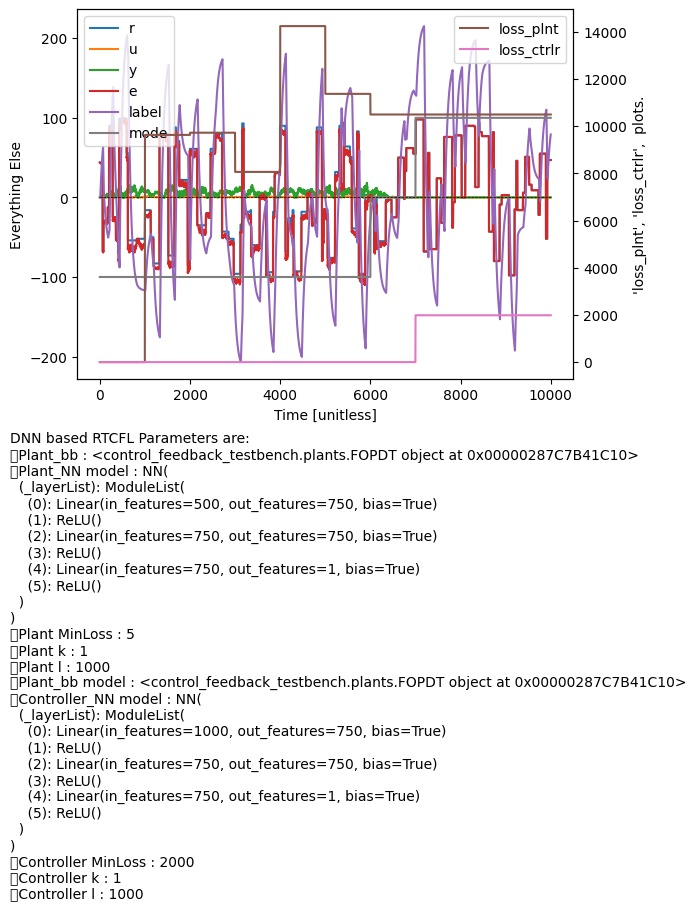
\includegraphics[width=\linewidth]{figures/output_plot_2022May03175654.jpg}
                \centering
                \caption{RTCFL-DNN circuit experiment result.}
                \label{dnnOut}
            \end{figure}
            \begin{figure}[h]
                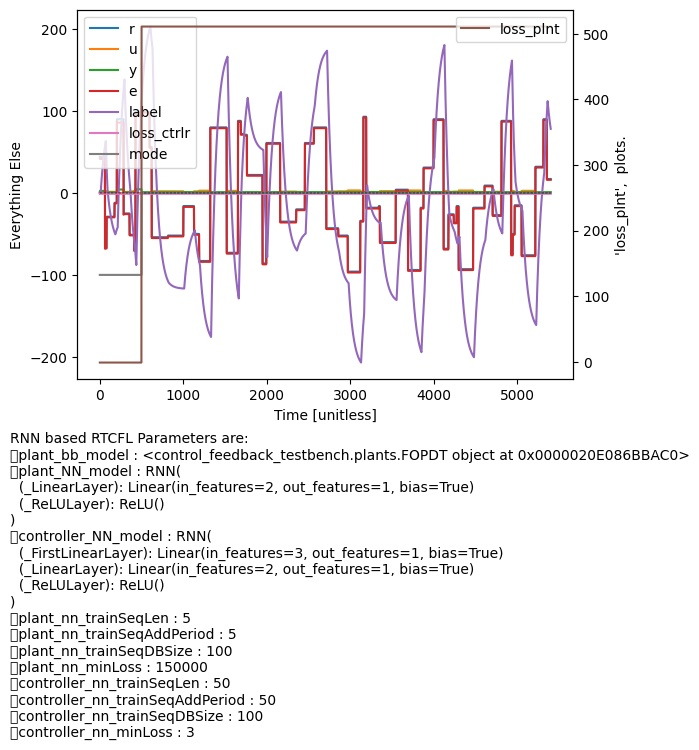
\includegraphics[width=\linewidth]{figures/output_plot_2022May03175716.jpg}
                \centering
                \caption{RTCFL-RNN circuit experiment result.}
                \label{rnnOut}
            \end{figure}
            \begin{figure}[h]
                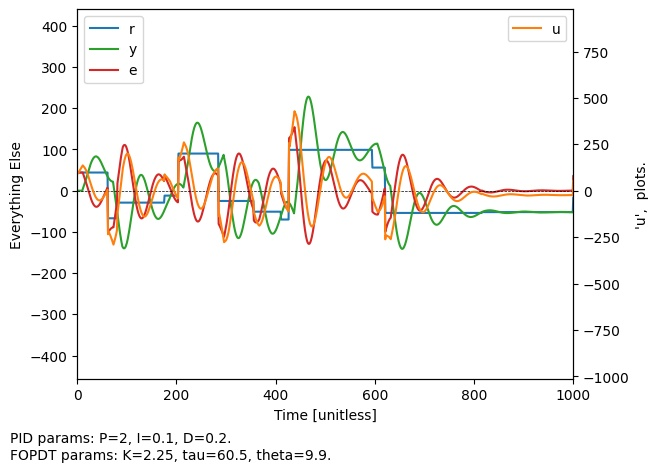
\includegraphics[width=\linewidth]{figures/output_plot_2022May04154543.jpg}
                \centering
                \caption{Static PID circuit experiment result.}
                \label{pidOut}
            \end{figure}

            As can be seen, in both the DNN and RNN RTCFL cases, the error ($e$) plots and the $controller_{NN}$ and
            $plant_{NN}$ plots (labelled $u$ and $y$ respectively) were extremely poor. Often times $NN$ outputs would
            be close to zero, implying the existence of vanished gradients. These problems were mostly attributed to the
            time spent on dialing in the various actor variables -- this aspect of `meta-tuning' proved to be extremely
            challenging. Given the plausibility of the RTCFL approach, it is reasonable to project potential successful
            and conclusive results in the future; that is given more testing and experimentation with different actor
            architectures (like LSTM's or Attention and Transformer Networks).

            For all the RTCFL's pros, there exists notable cons that require especially tuned networks to handle them.
            Firstly, the RTCFL would only be able to perform well in systems with really high sample rates, in order to
            collect enough data to achieve fast enough convergence. With the need for high sample rates, there is also a
            need for proportionally high temporal variation in input data in order to capture plant dynamics more
            generally. But with these high sample rates comes the need for more complex architectures and high memory
            requirements in order to `remember' enough past data to produce well informed outputs. For example, an RTCFL
            would probably not work in controllers for slow-changing high-thermal-capacity plants like in some
            over-sized industrial HVAC systems. Ultimately, these issues are a result of RTCFL's real-time nature and
            having to work with sparsely available data.

            Please see github here and here and here.
            % link github repository and quick rundown of where to find things.
 

    {\small
    \bibliographystyle{ieee_fullname}
    \bibliography{egbib}
    \nocite{*} % put this here to include all references without having to cite in the text
    }

    \section*{License}

        \doclicenseThis

\end{document}